\documentclass[a4paper,10pt]{article}
% \usepackage[latin1]{inputenc}
% \usepackage{ucs}
\usepackage[spanish]{babel}
\usepackage[utf8]{inputenc}
% \usepackage{bookman}
\usepackage{hyperref}
\usepackage{graphicx}
\selectlanguage{spanish}
\frenchspacing
\sloppy
\makeatletter

%% Metadatos del PDF.
\hypersetup{  
  pdftitle={System Integration and Administration with Free Software},
  pdfauthor={Miguel Vidal},
  pdfcreator={LaTeX},
  pdfproducer=PDFLaTeX,
  pdfsubject={Máster software libre},
}
%%


\title{\textbf{Práctica final}}			
\author{\textbf{Curso de arquitectura de servidores -- LibreSoft}}
\date{Marzo - Junio 2011}			


\begin{document}
\maketitle			
% \setcounter{tocdepth}{2}
% \tableofcontents

% \newpage

% \begin{abstract}

% \end{abstract}


\section*{Propósito}

El objetivo de la práctica final es consolidar los conocimientos adquiridos durante el curso y obtener el título propio.


\section{Descripción de la práctica}

La práctica consiste en \textbf{construir un cluster de alta disponibilidad en modo activo-activo} con un servidor web y una base de datos (típica estructura LAMP) y un almacenamiento compartido. He aquí el esquema:

% \bigskip

\begin{center}
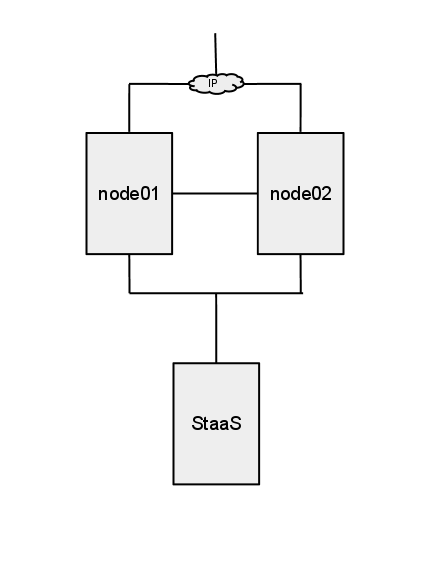
\includegraphics[width=75mm]{CASUL-Practica.png}
\end{center}

\begin{itemize}
\item \texttt{Node01} y \texttt{Node02} son los nodos del clúster HA (activo-activo). 
\item \texttt{StaaS} es un tercer nodo de almacenamiento compartido (NFS).
\end{itemize}


\subsection{Parte obligatoria}
\begin{itemize}
\item El cluster consistirá en 2 nodos unidos mediante una red dedicada para enviar el latido. El cluster será gestionado por \textbf{Linux-HA}. Se usará \textbf{Virtual\-Box} para crear los nodos del cluster y la red virtual dedicada.
\item El cluster gestionará dos servicios en Alta Disponibilidad: \textbf{MySQL} y \textbf{Apache}.
\item La configuración del cluster HA ha de ser \textbf{activo-activo}. 
\item Habrá un tercer nodo para exportar el almacenamiento por NFS; para este nodo, que ejerce de servidor NFS, se podrá utilizar el sistema operativo que se considere oportuno. El montaje y gestión de los directorios importados por NFS (el directorio que almacene la BD y el que albergue las páginas web) se deberán controlar mediante un agente de recurso del cluster HA.
\item Los agentes de recurso han de estar \textbf{agrupados} para una mejor gestión del cluster.
\item Entre el nodo de almacenamiento y los otros dos nodos habrá una red dedicada.
\item Habrá que prever cómo evitar el \textit{split-brain} si los enlaces de red que unen a los nodos entre sí cayesen.
\end{itemize}

\subsection{Parte optativa}

Aunque NO son requisitos para obtener el aprobado, se valorará positivamente incluir algunas de las siguientes mejoras por parte de quien desee ex\-peri\-mentar con otras tecnologías:

\begin{itemize}
\item Hacer el almacenamiento con iSCSI
\item Hacer el almacenamiento con DRBD (en este caso no es necesario un tercer nodo pero sí un agente de recurso adicional).
\item Utilizar un sistema operativo distinto de Linux para el almacenamiento:
	\begin{itemize}
	\item OpenIndiana para la exportación por NFS o iSCSI
	\item FreeNAS para la exportación por NFS o iSCSI
	\end{itemize}
\item Utilizar otras tecnologías de virtualización \textbf{libres} distintas a VirtualBox para construir la maqueta, como KVM, Xen o Qemu.
\end{itemize}

Cualquier otra mejora con tecnologías libres que se le ocurra al alumno (hayamos visto o no durante el curso) será bienvenida y se tendrá en cuenta a la hora de la calificación.


\section{Evaluación}

La evaluación consistirá en la presentación de la maqueta desarrollada en VirtualBox junto con unas preguntas que haremos los profesores para verificar que se ha entendido correctamente.

Además, el cluster deberá pasar la \textbf{batería de pruebas} que se adjunta en el \textbf{Anexo}.

La fecha de entrega será en uno de los días \textbf{21, 22 y 24 de junio} (dependiendo del turno escogido) en el Edificio Departamental II (despacho 106) del campus de Móstoles de la URJC (calle Tulipán s/n).

No hay posibilidad de segunda entrega. Se podrá recurrir al IRC (freenode, canal \texttt{\#casul}), al foro de Moodle o al email de los profesores desde la finalización del curso hasta esa fecha para resolver problemas.

\bigskip

\section*{Anexo - Batería de pruebas}

\footnotesize

\begin{tabular}{ | l || l |} \hline
\multicolumn{2}{|c|}{\bfseries Batería de pruebas}\\ \hline 
\multicolumn{1}{|c||}{\bfseries Caso}&\multicolumn{1}{c|}{\bfseries Resultado esperado}\\ \hline
Reiniciar máquina node01 & Inicio correcto con corosync activado \\ 
Reiniciar máquina node02 & Inicio correcto con corosync activado \\ \hline

Arrancar únicamente node01 & Todos los recursos levantan en node01 \\
Arrancar únicamente node02 & Todos los recursos levantan en nodo02 \\ \hline

Ambos nodos levantados, caída de node01 & Todos los recursos pasan a node02 \\
Ambos nodos levantados, caída de node02 & Todos los recursos pasan a node01 \\ \hline

Arrancado node01, levantar node02 & El grupo apache migra a node02 \\
Arrancado node02, levantar node01 & El grupo mysql migra a node01 \\ \hline

Tirar interfaz de cable cruzado & Ambos nodos online \\  
Tirar interfaz de servicio & Ambos nodos online \\ \hline

Matar proceso apache en node01 & Lo vuelve a levantar en node01 \\
Matar proceso mysql en node02 & Lo vuelve a levantar en node02 \\ \hline

\end{tabular}

\bigskip

\vspace{10mm}
\center{\scriptsize{Copyright
\copyright~2011 GSyC/Libresoft -- Miguel Vidal, José Castro \\
This work is licensed under a Creative Commons 
  Attribution 3.0 License, available at 
  \url{http://creativecommons.org/licenses/by/3.0/}




\end{document}



